\documentclass[a4paper,12pt]{report}
\usepackage[T2A]{fontenc}
\usepackage[utf8]{inputenc}
\usepackage[english,russian]{babel}
\usepackage{graphicx}
\usepackage{wrapfig}
\usepackage{mathtext} 				% русские буквы в фомулах
\usepackage{amsmath,amsfonts,amssymb,amsthm,mathtools} % AMS
\usepackage{icomma} % "Умная" запятая: $0,2$ --- число, $0, 2$ --- перечисление
\usepackage{capt-of}
\usepackage{appendix}
\usepackage{multirow}
\usepackage{hyperref}
\usepackage{floatrow}
\usepackage[left=2cm,right=2cm,
    top=2cm,bottom=2cm,bindingoffset=0cm]{geometry}
\usepackage{multicol} % Несколько колонок
\usepackage{gensymb}
\title{Отчёт по лабораторной работе № 5.10.1. 

Электронный парамагнитный резонанс}
\author{Плюскова Н.А. Б04-004 }
\date{\today}
\begin{document}
\maketitle
\section*{1. Аннотация}

В данной работе был исследован парамагнитный резонанс в молекуле ДФПГ, определен $g$-фактор электрона и измерена ширина линии ЭПР.

\section*{2. Теоретические сведения}
	Энергетический уровень электрона в присутствии магнитного поля с индукцией $B$ расщепляется на подуровня, расстояние между которыми равно 
	\begin{equation}
		\label{eq:dE}
		\Delta E = E_2 - E_1 = 2\mu B.
	\end{equation}
	Здесь $\mu$ -- абсолютная величина проекции магнитного момента на направление поля.
	
	Между этими двумя уровнями возможны переходы. Эти переходы могут возбуждаться внешним высокочастотным электромагнитным полем, если оно имеет нужную частоту и нужное направление.
	
	Резонансное значение частоты определяется из очевидной формулы:
	\begin{equation}
		\label{eq:resonans_omega}
		\hbar \omega_0 = \Delta E.
	\end{equation}

	При переходе с нижнего на верхний уровень энергии электрон поглощает квант электромагнитной энергии, а при обратном переходе такой же квант излучается. Возбуждение электронных резонансных переходов электромагнитным полем, имеющим частоту, определяемую формулой~(\ref{eq:resonans_omega}), носит название электронного парамагнитного резонанса (ЭПР).
	
	В настоящей работе необходимо получить сигнал ЭПР на кристаллическом дифенилпикрилгидразиле (ДФПГ) и определить значение $g$-фактора для электрона. Как известно, связь между магнитным моментом $\upmu$ электрона и его механическим моментом $\mathbf{M}$ выражается через гиромагнитное отношение $\gamma$ с помощью формулы
	\begin{equation}
		\label{eq:gyromagnit}
		\mu = \gamma \mathbf{M}.
	\end{equation}

	Используя соотношения (\ref{eq:dE})-(\ref{eq:gyromagnit}), нетрудно получить выражение для $g$-фактора через определяемые экспериментально величины:
	\begin{equation}
		\label{eq:g-faktor}
		\tag{$\star$}
		g = \frac{\hbar f_0}{\mu_\text{Б}B}.
	\end{equation}

\section*{3. Экспериментальная установка}
Образец (порошок ДФПГ) в стеклянной ампуле помещается внутрь катушки индуктивности входящей в состав колебательного контура. Входящий в состав контура конденсатор состоит из двух пластин, разделенных воздушным зазором, одна из пластин может перемещаться поворотом штока. Колебания в контуре возбуждаются антенной, соединённой с генератором частоты (ВЧ) Г4-116. Амплитуда колебаний поля в катушке индуктивности измеряется по наводимой в петле связи ЭДС индукции. Высокочастотные колебания ЭДС индукции в приёмном контуре детектируются диодом, измеряемая при помощи осциллографа низкочастотная огибающая этого сигнала пропорциональна квадрату амплитуды колебаний поля в катушке.
	\begin{figure}[h!]
		\begin{floatrow}
			\ffigbox[\FBwidth]{\caption{Схема установки.}\label{fig:ustanovka}}%
			{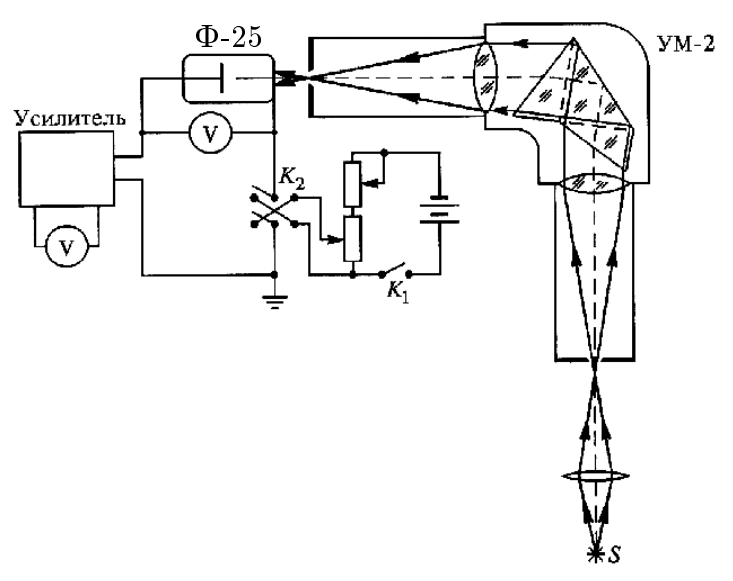
\includegraphics[scale=0.6]{ustanovka.pdf}}    
		\end{floatrow}
	\end{figure}
	
	Постоянной магнитное поле создаётся пропусканием тока от источника постоянного тока через основные катушки. При этом при помощи вольтметра измеряется падение напряжения на резисторе в цепи основных катушек. Переменное поле небольшой амплитуды создаётся подачей на модуляционные катушки напряжения с регулируемого трансформатора ЛАТР. Для измерения амплитуды колебаний переменного поля используется пробная катушка известной геометрии, подключенная к вольтметру.
	
\section*{4. Ход работы}
\subsection*{4.1 Параметры установки}
Запишем параметры катушек:

\begin{table}[H]
\begin{tabular}{|c|c|c|}
\hline
                      & $N$    & $d$, мм     \\ \hline
Основные катушки      & 5850 & -         \\ \hline
Модуляционные катушки & 1260 & -         \\ \hline
Пробная катушка       & 44   & 14,9$\pm$0,1 \\ \hline
\end{tabular}
\end{table}

Примерная частота колебательного контура: $f_{0} \approx 162$ МГц



\subsection*{4.2 Настройка ВЧ генератора и наблюдение сигнала резонансного поглощения}

Настроим генератор на частоту колебательного контура:
\begin{center}
    $f_{0} = (162,4\pm 0,2)$ Мгц
\end{center}

Подберем величину постоянного магнитного поля в катушках так, чтобы наблюдался сигнал резонансного поглощения. Для этого подадим на катушки достаточное напряжение.
		
Для более точной настройки и определения ширины линии резонансного поглощения будем наблюдать сигнал в $XY$-режиме. Запишем значение напряжения на резисторе в цепи основных катушек:
		\begin{equation*}
			U_0 = (178,7 \pm 1,1) \ \text{мВ}.
		\end{equation*}
		
\subsection*{4.3 Определение ширины линии ЭПР}
Определим ширину линии ЭПР (полуширина на на полувысоте линии резонансного поглощения):
		\begin{equation*}
			\Delta B =  \frac{A_{1/2}}{A_{\text{полн}}}\cdot2 B_\text{мод},
		\end{equation*}
		где $A_\text{полн}$ -- полный размах модулирующего поля, $A_{1/2}$ -- ширина кривой на полувысоте, $B_\text{мод}$ -- амплитуда модулирующего поля.
		\begin{equation*}
			\begin{gathered}
				A_\text{полн} = (10 \pm 0,2 ) \ \text{клетки}, \ A_{1/2} = (0,8 \pm 0,2) \ \text{клетки}
			\end{gathered}
		\end{equation*}

Измерим напряжение, возникающее внутри пробной катушки при внесение ее в поле основных катушек:

\begin{table}[H]
\begin{tabular}{|c|c|c|c|c|c|}
\hline
$V_{\text{мод}_{\text{перед}}}$,   мВ & $\sigma_{V_{\text{мод}_{\text{перед}}}}$,   мВ & $V_{\text{мод}_{\text{зад}}}$, мВ & $\sigma_{V_{\text{мод}_{\text{зад}}}}$,   мВ & $V_{\text{мод}_{\text{ср}}}$, мВ & $\sigma_{V_{\text{мод}_{\text{ср}}}}$, мВ \\ \hline
6,61            & 0,01                  & 6,48        & 0,01                & 6,55       & 0,01             \\ \hline
\end{tabular}
\end{table}

$B_{\text{мод}}$ найдем по формуле:
\begin{equation*}
    B_\text{мод} = \sqrt{2} \frac{2V_{\text{мод}_\text{ср}}}{\pi^2d^2N\nu} = (0,48\pm 0,03)\text{ мТл},
\end{equation*}
где $\nu = 400$Гц - частота модулирующего напряжения %(дана в лабнике).


Погрешность $B_{\text{мод}}$ считалась по формуле:

\begin{equation*}
    \sigma_{B_{\text{мод}}} = \sqrt{2} \frac{2}{\pi^2N\nu}\cdot \sqrt{(\frac{\sigma_{V_{\text{мод}_\text{ср}}}}{d^2})^2 + (\frac{\sigma_{d}\cdot V_{\text{мод}_\text{ср}}}{d^3})^2}
\end{equation*}

Тогда 
		\begin{equation*}
			\Delta B = (0,077\pm0,020) \text{ мТл},
		\end{equation*}
		
где погрешность $\Delta B$ была вычислена по формуле:

\begin{equation*}
			\sigma_{\Delta B} =  \sqrt{(\frac{2B_{\text{мод}}}{A_{\text{полн}}}\cdot \sigma_{A_{1/2}})^2 + (\frac{2B_{\text{мод}}\cdot A_{1/2}}{(A_{\text{полн}})^2}\cdot \sigma_{A_{\text{полн}}})^2 + (\frac{2A_{1/2}}{A_{\text{полн}}}\cdot \sigma_{B_{\text{мод}}})^2}
		\end{equation*}		
		
\subsection*{4.4 Калибровка основной катушки, нахождение $g$-фактора}
		
Определим связь между падением напряжения на резисторе в цепи основных катушек и магнитным полем в центре магнита:
		
\begin{table}[H]
\begin{tabular}{|c|c|c|c|c|c|c|c|}
\hline
$V$,   мВ   & $\sigma_{V},   мВ$ & $V_{\text{проб}}_{\text{перед}}$,   мВ & $\sigma_{V_{\text{проб}}_{\text{перед}}}$,   мВ & $V_{\text{проб}}_{\text{зад}}$,   мВ  & $\sigma_{V_{\text{проб}}_{\text{зад}}}$,   мВ & $V_{\text{ср}}$,   мВ   & $\sigma_{V_{\text{ср}}}$,   мВ \\ \hline
100,0 & 0,1       & 8,35   & 0,01         & 6,82  & 0,01       & 7,59  & 0,01      \\ \hline
115,2 & 0,1       & 9,56   & 0,01         & 7,82  & 0,01       & 8,69  & 0,01      \\ \hline
129,6 & 0,1       & 10,83  & 0,01         & 8,78  & 0,01       & 9,81  & 0,01      \\ \hline
145,0 & 0,1       & 11,90  & 0,10         & 9,68  & 0,01       & 10,79 & 0,05      \\ \hline
160,6 & 0,1       & 13,42  & 0,01         & 10,86 & 0,01       & 12,14 & 0,01      \\ \hline
174,4 & 0,1       & 14,51  & 0,01         & 11,76 & 0,01       & 13,14 & 0,01      \\ \hline
189,8 & 0,1       & 15,87  & 0,01         & 12,78 & 0,01       & 14,33 & 0,01      \\ \hline
205,4 & 0,3       & 17,03  & 0,01         & 13,84 & 0,01       & 15,44 & 0,01      \\ \hline
220,8 & 0,1       & 18,52  & 0,01         & 14,94 & 0,01       & 16,73 & 0,01      \\ \hline
234,8 & 0,1       & 19,47  & 0,01         & 15,73 & 0,01       & 17,60 & 0,01      \\ \hline
249,0 & 0,5       & 20,89  & 0,20         & 16,94 & 0,01       & 18,92 & 0,10      \\ \hline
\end{tabular}
\end{table}

Построим график $V(V_{\text{ср}})$:

	\begin{figure}[H]
		\centering
		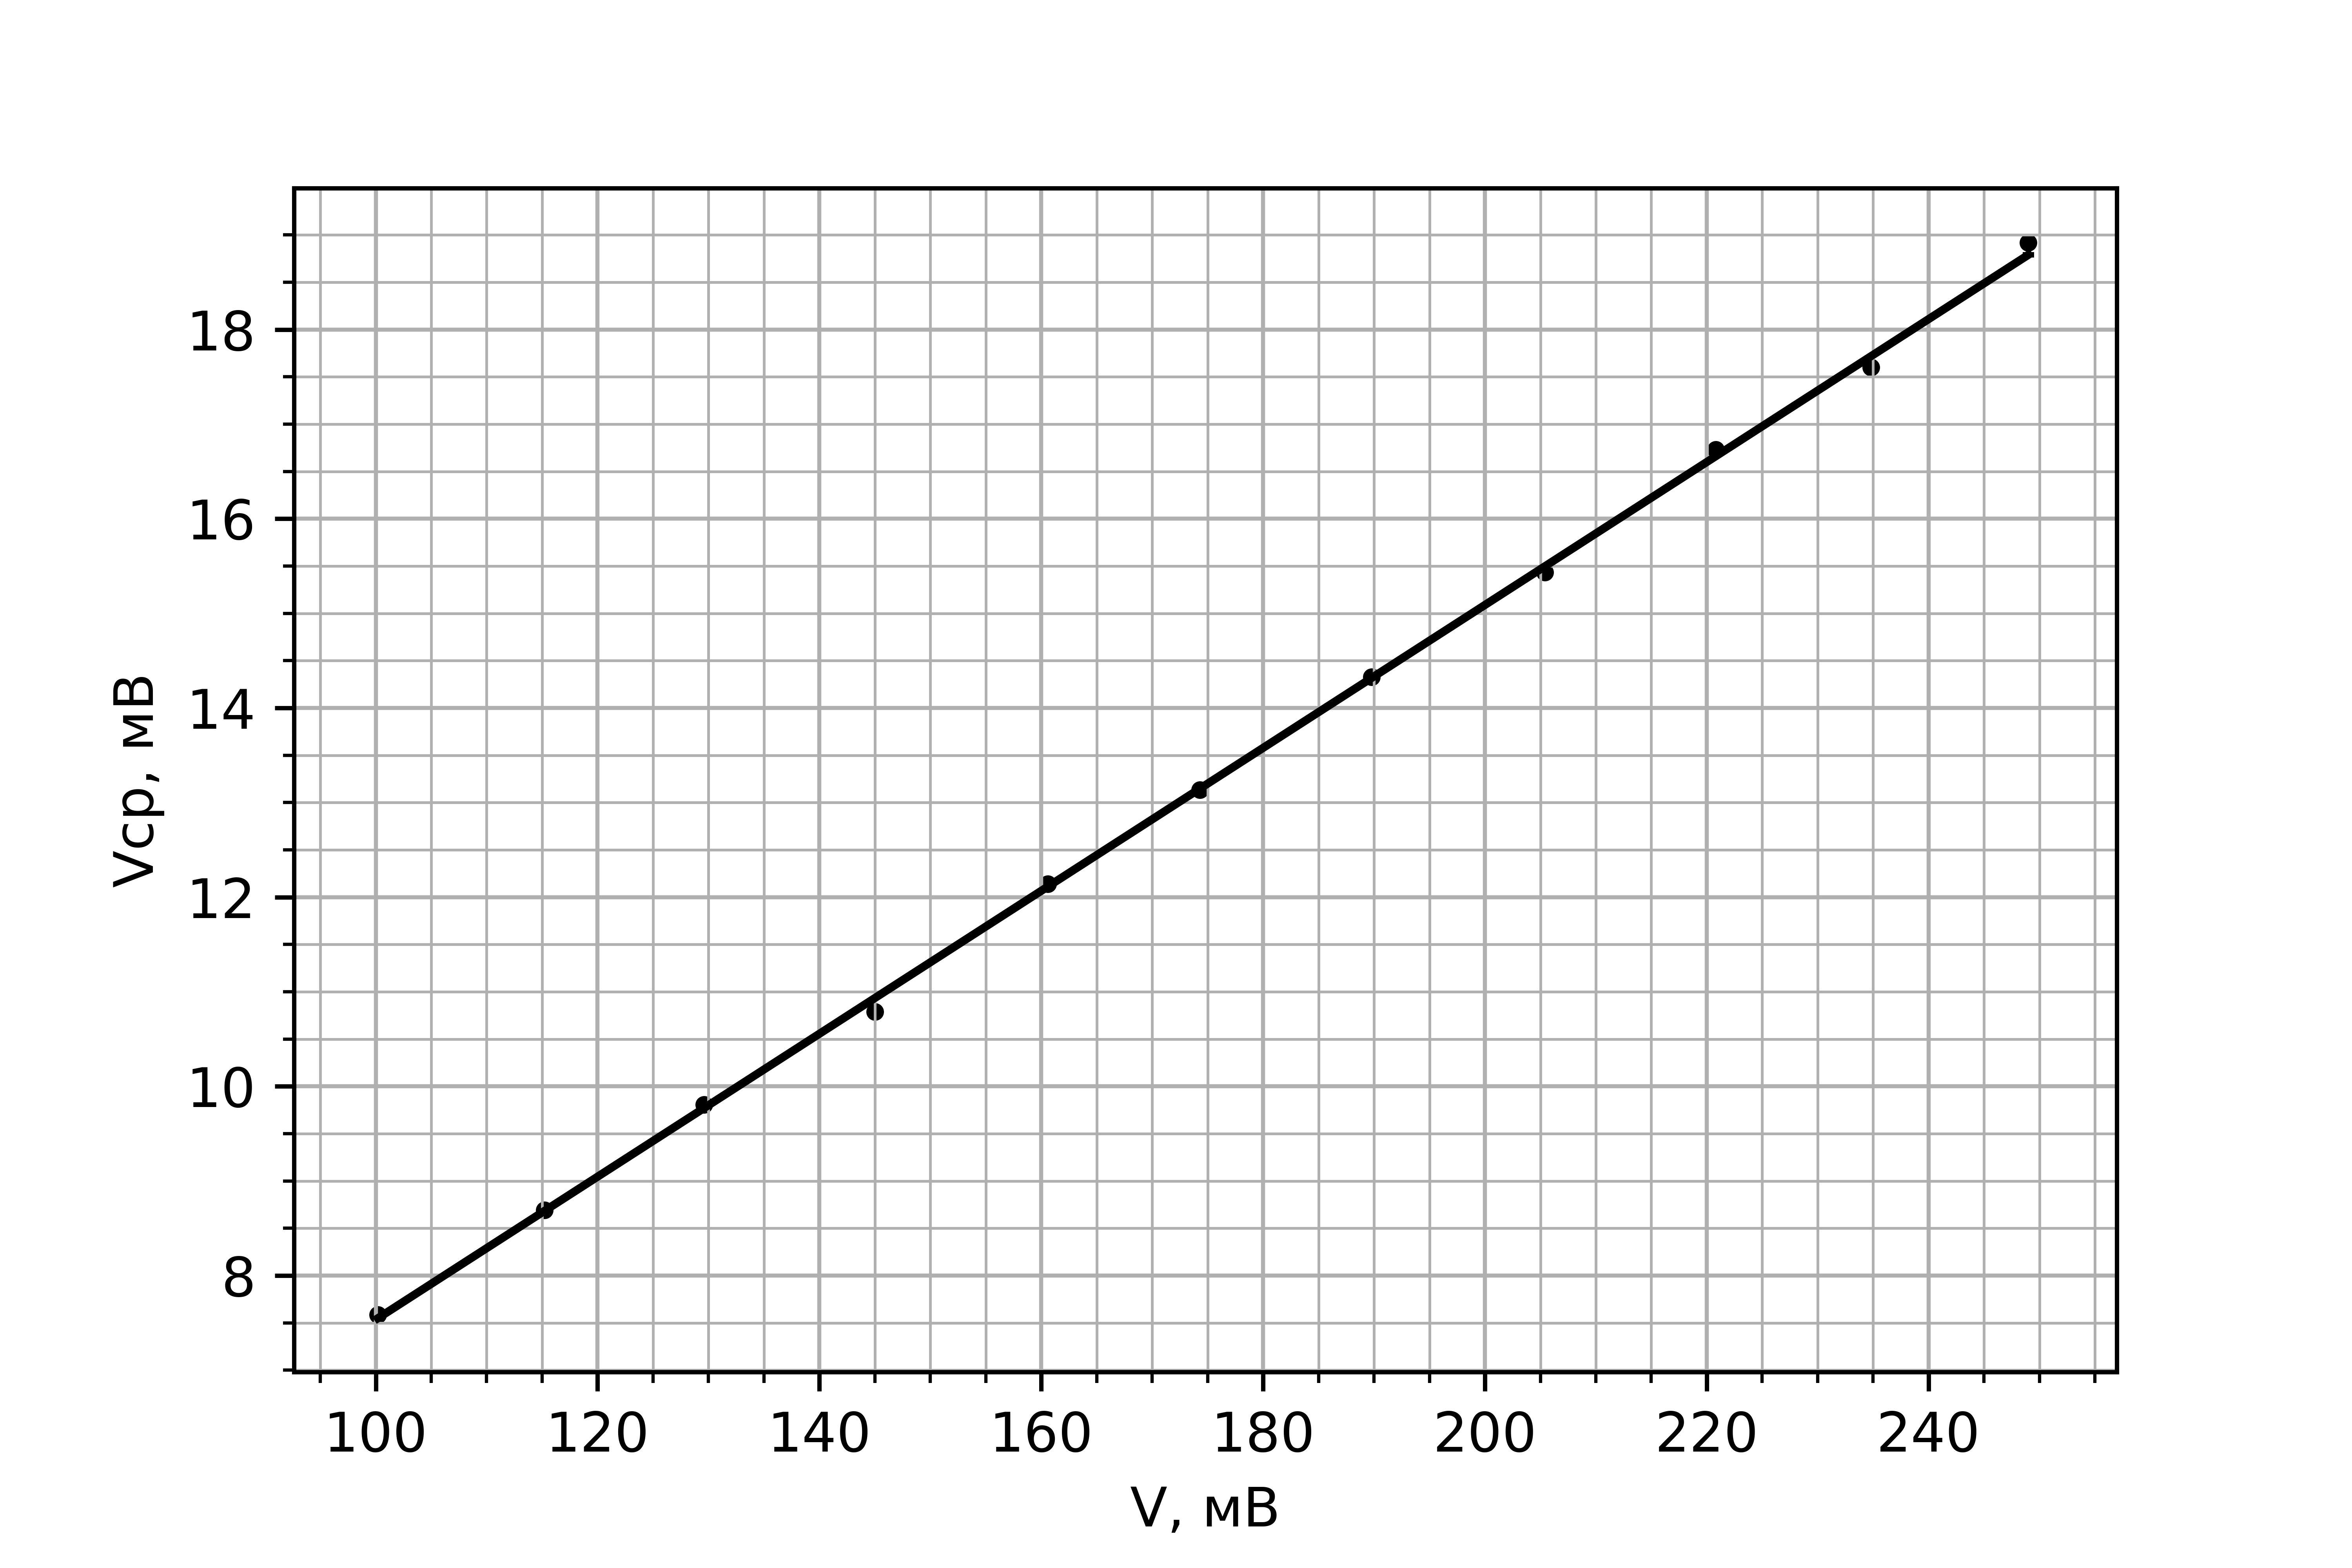
\includegraphics[width=0.7\linewidth]{V (Vср).png}
		\caption{Зависимость $V(V_{\text{ср}})$}
	\end{figure}
	
Из графика находим $U = (81,5\pm0,09)$ мВ при $V_{\text{мод}_{\text{ср}}} = (6,54 \pm 1,1)$ мВ.

%взяли большее и меньшее значение U_0 и по графику нашли U+- и как погрешность U взяли бОльшую разницу между значениями

Найдем $B_{0}$ по формуле:

\begin{equation}
B_0=\frac{4U}{\pi\omega d^2N_{\text{проб}}}=(4,49\pm0.11)\text{ мТл}
\end{equation}

%omega = 2Pi*nu

Погрешность $B_{0}$ была вычислена с помощью формулы:

\begin{equation*}
			\sigma_{B_{0}} = \frac{4}{\pi\omega N_{\text{проб}}}\cdot \sqrt{(\frac{\sigma_{U}}{d_{\text{проб}}^2})^2 + (\frac{2U\cdot\sigma_{d_{\text{проб}}}}{d_{\text{проб}}^3})^2}
		\end{equation*}		
		
Найдем $g$-фактор по формуле:

	\begin{equation}
		g = \frac{\hbar f_0}{\mu_\text{Б}B_{0}} = (2,58\pm0,07) 
	\end{equation}

Погрешность считали по формуле:
	\begin{equation}
		\sigma_{g} = \frac{\hbar}{\mu_\text{Б}} \cdot \sqrt{(\frac{\sigma_{f_{0}}}{B_{0}})^2 + (\frac{f_{0}\sigma_{B_{0}}}{B_{0}^2})^2}
	\end{equation}
	
Полученное значение отличается от теоретического ($g = 2$) на 29$\%$. Наибольшую погрешность в значение $g$-фактора вносят параметры пробной катушки, а также частота модулирующего напряжения, которые нам были даны.

Посчитаем добротность контура $Q$ по формуле:

	\begin{equation}
Q = \frac{\omega_{0}}{\Delta\omega} = \frac{\omega_{0}}{\frac{2\mu_{\text{Б}}g\Delta B}{\hbar}} = (64,79\pm7,63)
	\end{equation}
	
Погрешность считалась по формуле:
\begin{equation*}
    \sigma_{Q} = \frac{\hbar}{2\mu_{\text{Б}}}\sqrt{(\frac{\sigma_{\omega_{0}}}{g\Delta B})^2 + (\frac{\omega_{0}\sigma_{g}}{g^2 \Delta B})^2 + (\frac{\omega_{0}\sigma_{\Delta B}}{g\Delta B^2})^2}
\end{equation*}
	
\section*{5. Выводы}
В работе были получены значения амплитуды модулирующего поля $B_\text{мод}= (0,48\pm 0,03)\text{ мТл}$, ширины линий ЭПР $\Delta B = (0,077\pm0,020) \text{ мТл}$, а также значение $g$-фактора $g = (2,58\pm0,07) $, которое на 29 $\%$ больше теоретического

\end{document}
